\subsection*{engineering}
i assembled a simple ring modulator mockup in ltspice, which served to
illustrate the basic mechanics of making one. the difficulties in using a ring
modulator for direct upconversion is the input inductance and frequency -- the
modulating signal is coupled in through a transformer, which must operate both
at \rf and \ifreq.

fortunately, interchanging \rf and \ifreq leads to a still-working modulator! a
schematic is given in figure \ref{fig:ring-mod-spice}.

\begin{figure}[H]
	\centering
	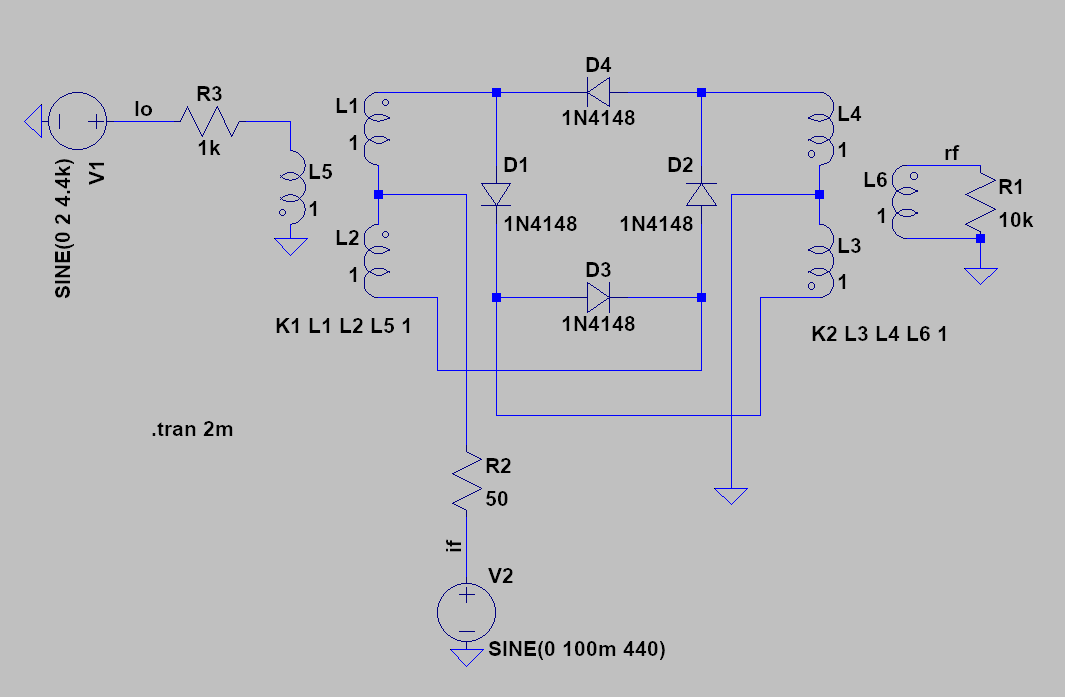
\includegraphics[width=.9\textwidth]{ring-mod-spice.png}
	\caption{ring modulator ltspice prototype}
	\label{fig:ring-mod-spice}
\end{figure}

the next step is to manage a \ssb transmitter. the basic process for \ssb
modulation is to modulate an in-phase \amp quadrature signal with the original
signal \amp its hilbert transform, respectively, as described in
\autocite{matlab-ssb}. this, however, requires a hilbert transformer\ldots\
which is apparently often implemented approximately with a filter, and in the
digital realm!

i decided to fiddle with \ssb modulation in octave to see if i could come up
with a good way to do it. the code may be found in
\localfile{../work/am-mod/code/ssb.m}.
